\documentclass{book} \usepackage{exsheets} \usepackage{xeCJK}
\usepackage{amsmath,amsfonts,amsthm,amssymb} \usepackage{bm}
\usepackage{hyperref} \usepackage{yhmath} \usepackage{caption}
\usepackage{pstricks-add} \usepackage{framed,mdframed}
\usepackage{graphicx,color} \usepackage{mathrsfs,xcolor}
\usepackage[all]{xy} \usepackage{fancybox}
\setCJKmainfont[BoldFont=SimHei]{SimSun} \SetupExSheets{
  counter-format = ch.se.qu , counter-within = section, solution/print
  = true }

\begin{document}
\chapter{高斯消去法}
\section{引言}
\section{高斯消去法举例}
\begin{question}
  用消元和反向代入解方程组
  \begin{align}
    2u-3v~~~~~~&=3\tag{1}\label{eq:1.2.1.1}\\
    4u-5v+w&=7\tag{2}\label{eq:1.2.1.2}\\
2u-v-3w&=5\tag{3}\label{eq:1.2.1.3}
  \end{align}
写出主元素,列出从其余的行中减去一行倍数的三个运算.
\end{question}
\begin{solution}
  \eqref{eq:1.2.1.2}-\eqref{eq:1.2.1.1}$\times 2$:
  \begin{equation}\tag{4}
    \label{eq:1.2.1.4}
    v+w=1
  \end{equation}
\eqref{eq:1.2.1.3}-\eqref{eq:1.2.1.1}$\times 1$:
\begin{equation}\tag{5}
  \label{eq:1.2.1.5}
  2v-3w=2.
\end{equation}
联立\eqref{eq:1.2.1.1},\eqref{eq:1.2.1.4},\eqref{eq:1.2.1.5}:
\begin{align*}
  2u-3v~~~~~~&=3\\
~~~~~~v+w&=1\\
~~~~~~2v-3w&=2
\end{align*}
\eqref{eq:1.2.1.5}-\eqref{eq:1.2.1.4}$\times 2$:
\begin{equation}\tag{6}
  \label{eq:1.2.1.6}
  -5w=0.
\end{equation}
联立\eqref{eq:1.2.1.1},\eqref{eq:1.2.1.4},\eqref{eq:1.2.1.6}:
\begin{align*}
  2u-3v~~~~~~&=3\\
~~~~~~v+w&=1\\
~~~~~~-5w&=0.
\end{align*}
解得$w=0,v=1,u=3$.主元素分别为$2,1,-5$.
\end{solution}
\begin{question}
  解方程组
  \begin{align}
    2u-v~~~~~~~~~~~~&=0\tag{1}\label{eq:1.2.2.1}\\
-u+2v-w~~~~~~&=0\tag{2}\label{eq:1.2.2.2}\\
-v+2w-z&=0\tag{3}\label{eq:1.2.2.3}\\
-w+2z&=5\tag{4}\label{eq:1.2.2.4}
  \end{align}
\end{question}
\begin{solution}
 \eqref{eq:1.2.2.2}-\eqref{eq:1.2.2.1}$\times -\frac{1}{2}$:
 \begin{equation}
   \label{eq:1.2.2.5}
   \tag{5}
\frac{3}{2}v-w=0.
 \end{equation}
联立\eqref{eq:1.2.2.1},\eqref{eq:1.2.2.5},\eqref{eq:1.2.2.3},\eqref{eq:1.2.2.4}:
\begin{align*}
  2u-v~~~~~~~~~~~~&=0\\
~~~~~~\frac{3}{2}v-w~~~~~~&=0\\
~~~~~~-v+2w-z&=0\\
~~~~~~~~~~~~-w+2z&=5.
\end{align*}
\eqref{eq:1.2.2.3}-\eqref{eq:1.2.2.5}$\times \frac{-2}{3}$:
\begin{equation}\tag{6}
  \label{eq:1.2.2.6}
  \frac{4}{3}w-z=0.
\end{equation}
联立
\eqref{eq:1.2.2.1},\eqref{eq:1.2.2.5},\eqref{eq:1.2.2.6},\eqref{eq:1.2.2.4}:
\begin{align*}
  2u-v~~~~~~~~~~~~&=0\\
\frac{3}{2}v-w~~~~~~&=0\\
~~~~~~~~~~~~\frac{4}{3}w-z&=0\\
~~~~~~~~~~~~-w+2z&=5.
\end{align*}
\eqref{eq:1.2.2.4}-\eqref{eq:1.2.2.6}$\times \frac{-3}{4}$:
$$
\frac{5}{4}z=5,
$$
解得$z=4,w=3,v=2,u=1$.
\end{solution}
\begin{question}
  试用消去法解方程组
  \begin{align}
    u+ v+w&=-2\label{eq:1.2.3.1}\tag{1}\\
   3u+3v-w&=6\label{eq:1.2.3.2}\tag{2}\\
    u- v+w&=-1\label{eq:1.2.3.3}\tag{3}
  \end{align}
遇到为零主元素时,请将它所在方程与下面的方程对调.然后继续进行消去.问:
第三个方程中$v$的系数$-1$换为什么数,消去法将不能进行.
\end{question}
\begin{solution}
 \eqref{eq:1.2.3.2}-\eqref{eq:1.2.3.1}$\times 3$:
 \begin{equation}\tag{4}
   \label{eq:1.2.3.4}
0\cdot u+0\cdot v -4w=12.
 \end{equation}
\eqref{eq:1.2.3.3}-\eqref{eq:1.2.3.1}:
\begin{equation}
  \label{eq:1.2.3.5}
  \tag{5}
0\cdot u-2v+0\cdot w=1.
\end{equation}
联立方程\eqref{eq:1.2.3.5}和方程\eqref{eq:1.2.3.4},得
\begin{align*}
  0\cdot u-2v+0\cdot w&=1\\
 0\cdot u+0\cdot v-4w&=12.
\end{align*}
解得$v=\frac{-1}{2}$,$w=-3$,$u=\frac{3}{2}$.将第三个方程中$v$的系数
$-1$换为$1$,消去法将不能进行.
\end{solution}
\begin{question}
$n=2$时$P=2$.试列出用消去法解方程组
\begin{align}
au+bv&=0  \label{eq:1.2.4.1}
  \tag{1}\\
cu+dv&=1\label{eq:1.2.4.2}\tag{2}
\end{align}
时,对左端所进行的运算.
\end{question}
\begin{solution}
\begin{itemize}
\item 当$a\neq 0$时,\eqref{eq:1.2.4.2}-\eqref{eq:1.2.4.1}$\times \frac{c}{a}$:
\begin{equation}
  \label{eq:1.2.4.3}
  \tag{3}
(d-\frac{bc}{a})v=1.
\end{equation}
联立方程\eqref{eq:1.2.4.1},\eqref{eq:1.2.4.3},可得
\begin{align*}
  au+bv&=0\\
 (d-\frac{bc}{a})v&=1.
\end{align*}
若$ad-bc=0$,则$v$无解.即当$a\neq 0,ad-bc=0$时,方程组无解;若$ad-bc\neq
0$,则$v=\frac{a}{ad-bc}$,$u=\frac{-b}{ad-bc}$.即当$a\neq
  0,ad-bc\neq 0$时,方程组有唯一解
  $u=\frac{-b}{ad-bc}$,$v=\frac{a}{ad-bc}$.
\item 当$a=0$时,若$c\neq 0$,则交换方程\eqref{eq:1.2.4.1}和方程
  \eqref{eq:1.2.4.2}的顺序,得到
  \begin{align*}
    cu+dv&=1\\
        bv&=0
  \end{align*}
此时若$b\neq 0$,则$v=0$,$u=\frac{1}{c}$;若$b=0$,则方程组有无数个解.\\

反之,若$c=0,d=0$,则无解.若$c=0,d\neq 0,b=0$,则有无穷解.若$c=0,d\neq
0,b\neq 0$,无解.
\end{itemize}
\end{solution}
\begin{question}
  设解线性方程组所需运算次数为$\frac{n^3}{3}$,计算机的速度为每秒一百万
  次,收费标准为每小时$1000$元.试问化$1$元钱可以解多大的方程组,化
  $1000$元可以解多大的方程组?
\end{question}
\begin{solution}
  花一元钱,可以使用$\frac{1}{1000}$小时,即$3.6$秒.此时计算机可以算
  $3.6\times 10^7$次.由$\frac{n^3}{3}=3.6\times 10^7$解得$n\approx
  476$.花$1000$元,可以使用$1$小时,即$3600$秒.此时计算机可以算
  $3.6\times 10^{10}$次.由$\frac{n^3}{3}=3.6\times 10^{10}$,解得
  $n\approx 4762$.
\end{solution}
\begin{question}
略.
\end{question}
\begin{question}
  试用消去法解
  \begin{align}
u+v+w&=6   \tag{1}\label{eq:1.2.7.1}\\
u+2v+2w&=11\tag{2}\label{eq:1.2.7.2}\\
2u+3v-4w&=3\tag{3}\label{eq:1.2.7.3}
  \end{align}
\end{question}
\begin{solution}
  \eqref{eq:1.2.7.2}-\eqref{eq:1.2.7.1}:
  \begin{equation}
    \label{eq:1.2.7.4}
    \tag{4}
v+w=5.
  \end{equation}
\eqref{eq:1.2.7.3}-\eqref{eq:1.2.7.1}$\times 2$:
\begin{equation}
  \label{eq:1.2.7.5}\tag{5}
  v-6w=-9.
\end{equation}
联立方程\eqref{eq:1.2.7.1},\eqref{eq:1.2.7.4},\eqref{eq:1.2.7.5},可得
\begin{align*}
  u+v+w&=6\\
~~~~~~v+w&=5\\
~~~~~~v-6w&=-9\\
\end{align*}
\eqref{eq:1.2.7.5}-\eqref{eq:1.2.7.4}:
\begin{equation}\label{eq:1.2.7.6}\tag{6}
  -7w=-14.
\end{equation}
联立方程\eqref{eq:1.2.7.1},\eqref{eq:1.2.7.4},\eqref{eq:1.2.7.6},可得
\begin{align*}
  u+v+w&=6\\
~~~~~~v+w&=5\\
~~~~~~~~~~~~~~-7w&=-14.
\end{align*}
解得$w=2,v=3,u=1$.
\end{solution}
\section{矩阵和矩阵乘法}
\begin{question}
  先用$A$的单个元素再利用$A$的整列计算乘积
$$
Ax=
\begin{pmatrix}
  4&0&1\\
  0&1&0\\
  4&0&1
\end{pmatrix}
\begin{pmatrix}
  3\\
  4\\
  5\\
\end{pmatrix}.
$$
\end{question}
\begin{solution}
  利用$A$的单个元素计算乘积略.利用$A$的整列计算乘积:
$$
Ax=3
\begin{pmatrix}
  4\\
  0\\
  4
\end{pmatrix}+4
\begin{pmatrix}
  0\\
  1\\
  0
\end{pmatrix}+5
\begin{pmatrix}
  1\\
  0\\
  1\\
\end{pmatrix}=
\begin{pmatrix}
  17\\
  4\\
  17
\end{pmatrix}.
$$
\end{solution}
\begin{question}
  试计算乘积
$$
Ax=
\begin{pmatrix}
  1&2\\
  3&-3\\
  0&4\\
  0&1
\end{pmatrix}
\begin{pmatrix}
  1\\
  -1
\end{pmatrix}\mbox{和}
\begin{pmatrix}
  -4&1&3
\end{pmatrix}
\begin{pmatrix}
  -4\\
  1\\
  3\\
\end{pmatrix}.
$$
如果$A$是$m\times n$矩阵,$x$是$n$维向量,试问乘积$Ax$的行数列数各为
几?
\end{question}
\begin{solution}
$$
  \begin{pmatrix}
    1&2\\
    3&-3\\
    0&4\\
    0&1
  \end{pmatrix}
  \begin{pmatrix}
    1\\
    -1
  \end{pmatrix}=1\cdot
  \begin{pmatrix}
    1\\
    3\\
    0\\
    0\\
  \end{pmatrix}+(-1)\cdot
  \begin{pmatrix}
    2\\
    -3\\
    4\\
    1\\
  \end{pmatrix}=
  \begin{pmatrix}
    -1\\
    6\\
    -4\\
    -1
  \end{pmatrix},
$$
$$
\begin{pmatrix}
  -4&1&3
\end{pmatrix}
\begin{pmatrix}
  -4\\
  1\\
  3
\end{pmatrix}=\begin{pmatrix}(-4)\times (-4)+1\times 1+3\times
  3\end{pmatrix}=\begin{pmatrix}26\end{pmatrix}.
$$
如果$A$是$m\times n$矩阵,$x$是$n$维向量,则$Ax$的行数为$m$行,列数
为$1$列.
\end{solution}
\begin{question}
  假定某年年初与年末相比较
  \begin{itemize}
  \item 原来住在美国加州的人中$80\%$留在加州,$20\%$迁出加州.
  \item 原来住美国国内加州以外的人中$90\%$仍留在加州以外,$10\%$迁入加
    州.
  \end{itemize}
  试根据以上两条将下列问题用“矩阵形式”表达出来,并求解.
  \begin{itemize}
  \item 年初美国加州内外人数分别为$30$和$200$(单位百万,下同),问年末州
    内外人数各若干?
  \item 问年初人口是怎样一种分布时,年末人口分布不变,换句话说,要求年
    末时加州内外人口数$u,v$与年初时相同,年初时$u$和$v$应是多少?
  \end{itemize}
\end{question}
\begin{solution}
  设年初加州人口为$a_{1}$,美国国内加州之外的人口为$b_{1}$.则在年末,加
  州人口$a_{2}$为
$$
a_{2}=0.8a_{1}+0.1b_{1},
$$
加州之外的人口$b_2$为
$$
b_2=0.2a_{1}+0.9b_{1}.
$$
写成矩阵形式,即
$$
\begin{pmatrix}
  a_2\\
  b_2
\end{pmatrix}=
\begin{pmatrix}
  0.8&0.1\\
  0.2&0.9
\end{pmatrix}
\begin{pmatrix}
  a_{1}\\
  b_{1}\\
\end{pmatrix}.
$$
\begin{itemize}
\item 当$a_1=30,b_1=200$时,易得
$$
\begin{pmatrix}
  a_2\\
  b_2
\end{pmatrix}=
\begin{pmatrix}
  0.8&0.1\\
  0.2&0.9
\end{pmatrix}
\begin{pmatrix}
  30\\
  200
\end{pmatrix}=
\begin{pmatrix}
  44\\
  186
\end{pmatrix}.
$$
所以年末加州内外人口分别为$44$万和$186$万.
\item 年末人口分布不变,意味着
$$
\begin{pmatrix}
  a_2\\
  b_2
\end{pmatrix}=
\begin{pmatrix}
  0.8&0.1\\
  0.2&0.9
\end{pmatrix}
\begin{pmatrix}
  a_{1}\\
  b_{1}\\
\end{pmatrix}=
\begin{pmatrix}
  a_1\\
  b_1\\
\end{pmatrix},
$$
即
$$
\begin{pmatrix}
  0.8-1&0.1\\
  0.2&0.9-1
\end{pmatrix}
\begin{pmatrix}
  a_1\\
  b_1\\
\end{pmatrix}=
\begin{pmatrix}
  0\\
  0\\
\end{pmatrix}.
$$
解得$b_1=2a_1$.即当年初美国国内加州外人口是加州内人口的两倍时,年末人口
分布不变.这在直观上也是好理解的.
\end{itemize}
\end{solution}
\begin{question}
  略.
\end{question}
\begin{question}
  试求$E$与$A$的乘积
$$
E=
\begin{pmatrix}
  1&0&0\\
  -2&1&0\\
  1&0&1
\end{pmatrix},A=
\begin{pmatrix}
  2&1&1\\
  4&1&0\\
  -2&2&1
\end{pmatrix}.
$$
\end{question}
\begin{solution}
  \begin{align*}
    \begin{pmatrix}
      1&0&0\\
      -2&1&0\\
      1&0&1
    \end{pmatrix}
           \begin{pmatrix}
             2&1&1\\
             4&1&0\\
             -2&2&1
           \end{pmatrix}&=
                          \begin{pmatrix}
                            1&0&0\\
                            -2&1&0\\
                            1&0&1
                          \end{pmatrix}
                                 \begin{pmatrix}
                                   2&0&0\\
                                   4&0&0\\
                                   -2&0&0
                                 \end{pmatrix}+\begin{pmatrix}
                                   1&0&0\\
                                   -2&1&0\\
                                   1&0&1
                                 \end{pmatrix}
                                        \begin{pmatrix}
                                          0&1&0\\
                                          0&1&0\\
                                          0&2&0
                                        \end{pmatrix}\\&+ \begin{pmatrix}
                                          1&0&0\\
                                          -2&1&0\\
                                          1&0&1
                                        \end{pmatrix}
                                               \begin{pmatrix}
                                                 0&0&1\\
                                                 0&0&0\\
                                                 0&0&1
                                               \end{pmatrix}\\
       &=
         \begin{pmatrix}
           2&0&0\\
           0&0&0\\
           0&0&0
         \end{pmatrix}+
                \begin{pmatrix}
                  0&1&0\\
                  0&-1&0\\
                  0&3&0
                \end{pmatrix}+
                       \begin{pmatrix}
                         0&0&1\\
                         0&0&-2\\
                         0&0&2
                       \end{pmatrix}\\&=
                                        \begin{pmatrix}
                                          2&1&1\\
                                          0&-1&-2\\
                                          0&3&2
                                        \end{pmatrix}.
  \end{align*}
\end{solution}
\begin{question}
  试求$E$和$A$的积
$$
E=
\begin{pmatrix}
  1&0&0\\
  -2&1&0\\
  -5&3&1
\end{pmatrix},A=
\begin{pmatrix}
  2&1&1\\
  4&1&0\\
  -2&2&1
\end{pmatrix}.
$$
\end{question}
\begin{solution}
  我们先来确定矩阵$EA$的第一列:
$$
2
\begin{pmatrix}
  1\\
  -2\\
  -5
\end{pmatrix}+4
\begin{pmatrix}
  0\\
  1\\
  3\\
\end{pmatrix}+(-2)
\begin{pmatrix}
  0\\
  0\\
  1
\end{pmatrix}=
\begin{pmatrix}
  2\\
  0\\
  0
\end{pmatrix}.
$$
再确定矩阵$EA$的第二列:
$$
1
\begin{pmatrix}
  1\\
  -2\\
  -5
\end{pmatrix}+1
\begin{pmatrix}
  0\\
  1\\
  3
\end{pmatrix}+2
\begin{pmatrix}
  0\\
  0\\
  1
\end{pmatrix}=
\begin{pmatrix}
  1\\
  -1\\
  0
\end{pmatrix}.
$$
最后确定矩阵$EA$的第三列:
$$
1\cdot
\begin{pmatrix}
  1\\
  -2\\
  -5
\end{pmatrix}+0\cdot
\begin{pmatrix}
  0\\
  1\\
  3
\end{pmatrix}+1\cdot
\begin{pmatrix}
  0\\
  0\\
  1
\end{pmatrix}=
\begin{pmatrix}
  1\\
  -2\\
  -4
\end{pmatrix}.
$$
所以矩阵$EA$为
$$
\begin{pmatrix}
  2 &1  &1 \\
  0 &-1 &-2\\
  0 &0  &-4\\
\end{pmatrix}.
$$
\end{solution}
\begin{question}
  试将$1\times 2$矩阵$E=
  \begin{pmatrix}
    1&-4
  \end{pmatrix}
  $与$2\times 1$矩阵$A=
  \begin{pmatrix}
    4\\
    1
  \end{pmatrix}
  $相乘,当$E$是$l\times
  m$矩阵,$A$是$m\times n$矩阵时,为得到乘积$EA$所需进行的单个乘法
  为$lmn$个.试说明理由.
\end{question}
\begin{solution}
$$
EA=
\begin{pmatrix}
  4\times 1+1\times(-4)
\end{pmatrix}=
\begin{pmatrix}
  0
\end{pmatrix}
$$
每确定矩阵$EA$的特定的一列都需要乘$ml$次乘法,共需要确定$n$列,因此为了
得到矩阵$EA$需要$lmn$次乘法.
\end{solution}
\begin{question}
  试将下面的$3\times 2$矩阵$E$与$2\times 1$矩阵$A$相乘
$$
E=
\begin{pmatrix}
  8&-3\\
  -5&2\\
  1&0
\end{pmatrix},A=
\begin{pmatrix}
  2\\
  1
\end{pmatrix}.
$$
\end{question}
\begin{solution}
$$
EA=2
\begin{pmatrix}
  8\\
  -5\\
  1
\end{pmatrix}+1
\begin{pmatrix}
  -3\\
  2\\
  0
\end{pmatrix}=
\begin{pmatrix}
  13\\
  -8\\
  2
\end{pmatrix}.
$$
\end{solution}
\begin{question}
  试对下面的$A,B,C$验证结合律
$$
A=
\begin{pmatrix}
  1&0&0\\
  0&1&0\\
  1&0&1
\end{pmatrix},B=
\begin{pmatrix}
  1&0&0\\
  -2&1&0\\
  0&0&1
\end{pmatrix},C=
\begin{pmatrix}
  2&1&1\\
  4&1&0\\
  -2&2&1
\end{pmatrix}.
$$
\end{question}
\begin{solution}
  与其验证矩阵乘法的结合律对于特定的矩阵成立,不如来理解矩阵乘法的本质.矩
  阵乘法,其实就是从线性映射的复合而来的.以$2\times 2$矩阵为
  例,设$\alpha=(\mathbf{e}_1,\mathbf{e}_2)$是$\mathbf{R}^2$的一组有序基
  底(ordered
  basis),向量$\mathbf{v}$在该有序基下的坐标
  为$(x,y)$,即$[\mathbf{v}]^{\alpha}=
  \begin{pmatrix}
    x\\
    y
  \end{pmatrix}
  $.矩阵
$$
[T_{1}]_{\alpha}^{\alpha}=
\begin{pmatrix}
  a_{11}&a_{12}\\
  a_{21}&a_{22}
\end{pmatrix},[T_{2}]_{\alpha}^{\alpha}=
\begin{pmatrix}
  b_{11}&b_{12}\\
  b_{21}&b_{22}
\end{pmatrix}.
$$
向量$\mathbf{v}$在矩阵$[T_{1}]_{\alpha}^{\alpha}$的作用下变成的向量在有
序基$\alpha$下的坐标为
\begin{equation}\label{eq:1.3.9.1}\tag{1}
  \begin{pmatrix}
    a_{11}&a_{12}\\
    a_{21}&a_{22}
  \end{pmatrix}
  \begin{pmatrix}
    x\\
    y
  \end{pmatrix}=
  \begin{pmatrix}
    a_{11}x+a_{12}y\\
    a_{21}x+a_{22}y
  \end{pmatrix}.
\end{equation}
从基底的观点来看,矩阵$[T_1]_{\alpha}^{\alpha}$把基向量$\mathbf{e}_1$变
为$a_{11}\mathbf{e}_1+a_{21}\mathbf{e}_2$,把基向
量$\mathbf{e}_2$变为$a_{12}\mathbf{e}_1+a_{22}\mathbf{e}_2$,用表格表示
即
\begin{center}
  \begin{tabular}{|c|c|c|}
    $[T_1]_{\alpha}^{\alpha}$ & $\mathbf{e}_1$& $\mathbf{e}_{2}$\\
    $\mathbf{e}_1$ & $a_{11}$ & $a_{12}$ \\
    $\mathbf{e}_2$ & $a_{21}$ & $a_{22}$ \\
  \end{tabular}
\end{center}
所以矩阵$[T_1]_{\alpha}^{\alpha}$把向量$\mathbf{v}$变为
$$
\mathbf{v}'=x(a_{11}\mathbf{e}_1+a_{21}\mathbf{e}_2)+y(a_{12}\mathbf{e}_1+a_{22}\mathbf{e}_2)=(a_{11}x+a_{12}y)\mathbf{e}_1+(a_{21}x+a_{22}y)\mathbf{e}_2,
$$
这就是矩阵表达式\eqref{eq:1.3.9.1}的线性变换解释.\\

这样,就可以从线性变换的观点来理解线性方程组
$$
\begin{cases}
  a_{11}x+a_{12}y=c_1\\
  a_{21}x+a_{22}y=c_2
\end{cases},
$$
意思就是,求满足条件的向量$\mathbf{v}$,使得向量$\mathbf{v}$经过线性映
射$[T_1]_{\alpha}^{\alpha}$的作用后,会变成向量
$c_1\mathbf{e}_1+c_2\mathbf{e}_2$.\\

如果向量$\mathbf{v}$先经过矩阵$[T_1]_{\alpha}^{\alpha}$的作用,变成向
量$\mathbf{v}'$,向量$\mathbf{v}'$再经过矩阵$[T_2]_{\alpha}^{\alpha}$的
作用,变为向量$\mathbf{v}''$.那么向量$\mathbf{v}''$在有序基$\alpha$下的
坐标是什么样的呢?经过简单的心算,可以得到如下表格
\begin{center}
  \begin{tabular}{|c|c|c|}
    $[T_{2}]_{\alpha}^{\alpha}\circ[T_1]_{\alpha}^{\alpha}$ & $\mathbf{e}_1$& $\mathbf{e}_{2}$\\
    $\mathbf{e}_1$ & $b_{11}a_{11}+b_{12}a_{21}$ & $b_{11}a_{12}+b_{12}a_{22}$ \\
    $\mathbf{e}_2$ & $b_{21}a_{11}+b_{22}a_{21}$ & $b_{21}a_{12}+b_{22}a_{22}$ \\
  \end{tabular}
\end{center}
这符合矩阵$[T_{2}]_{\alpha}^{\alpha}[T_1]_{\alpha}^{\alpha}$的乘法规则.既
然矩阵的乘法无非就是线性变换的复合,而映射的复合满足结合律,因此矩阵的
乘法自然也满足结合律.
\end{solution}
\begin{question}
  试证,如果$A=
  \begin{pmatrix}
    a&b\\
    c&d
  \end{pmatrix}
  $与矩阵
$$
B=
\begin{pmatrix}
  1&0\\
  0&0
\end{pmatrix}
\mbox{和}C=
\begin{pmatrix}
  0&1\\
  0&0
\end{pmatrix}
$$
相乘时都可交换,则$A$必为单位矩阵的倍数,即$a=d,b=c=0$.再证这样的$A$与
任何$2\times 2$矩阵相乘时都是可交换的,也即只有这样的矩阵才具有这种性质.
\end{question}

\begin{solution}
  $$ 
  AB=
  \begin{pmatrix}
    a&b\\
    c&d
  \end{pmatrix}
  \begin{pmatrix}
    1&0\\
    0&0
  \end{pmatrix}=
  \begin{pmatrix}
    a&0\\
    c&0
  \end{pmatrix},BA=
  \begin{pmatrix}
    1&0\\
    0&0
  \end{pmatrix}
  \begin{pmatrix}
    a&b\\
    c&d
  \end{pmatrix}=
  \begin{pmatrix}
    a&b\\
    0&0
  \end{pmatrix}.
 $$
 可见,若$AB=BA$,则$b=c=0$.
$$
AC=
\begin{pmatrix}
  a&b\\
  c&d
\end{pmatrix}
\begin{pmatrix}
  0&1\\
  0&0
\end{pmatrix}=
\begin{pmatrix}
  0&a\\
  0&c
\end{pmatrix},CA=
\begin{pmatrix}
  0&1\\
  0&0
\end{pmatrix}
\begin{pmatrix}
  a&b\\
  c&d
\end{pmatrix}=
\begin{pmatrix}
  c&d \\
  0&0
\end{pmatrix}.
$$
可见,若$AC=CA$,则$c=0,d=1$.若同时满足$AB=BA,AC=CA$,则$a=d,b=c=0$.可
见,$A=kI$,其中$I$是单位矩阵.而且,容易验证,此时对于任意$2\times 2$矩
阵$M$来说,$AM=MA=kM$.
\end{solution}
\begin{question}
  试举出具有下列性质的$2\times 2$矩阵
  \begin{itemize}
  \item $A^2=-I$,$A$的元素都是实数;
  \item $B^2=0,B\neq 0$;
  \item {\color{red}$CD=-DC$,$CD\neq 0$}
  \item $EF=0$,$E,F$的元素全都不为零.
  \end{itemize}
\end{question}
\begin{solution}
  \begin{itemize}
  \item
$$
A=
\begin{pmatrix}
  \cos \frac{\pi}{2}&-\sin \frac{\pi}{2}\\
  \sin \frac{\pi}{2}&\cos \frac{\pi}{2}
\end{pmatrix}=
\begin{pmatrix}
  0&-1\\
  1&0
\end{pmatrix}.
$$
\item
$$
B=
\begin{pmatrix}
  0&0\\
  1&0\\
\end{pmatrix}.
$$
\item 书上给出的答案是$C=
  \begin{pmatrix}
    0&1\\
    1&0
  \end{pmatrix},D=
  \begin{pmatrix}
    0&1\\
    -1&0
  \end{pmatrix}.
  $我能提供的是对$CD=-DC$的解释.不妨设$C,D$都是可逆矩阵,
  则$D=C^{-1}(-D)C$.即$D$和$-D$是相似矩阵.即要选取一个线性变换和两个不
  同的基底,这个线性变换在两个不同基底下的矩阵是相反矩阵.
\item
$$
E=
\begin{pmatrix}
  1&-1\\
  -1&1
\end{pmatrix},F=
\begin{pmatrix}
  1&1\\
  1&1
\end{pmatrix}.
$$
\end{itemize}
\end{solution}
\begin{question}
  问下列命题成立否,不成立的请举例
  \begin{itemize}
  \item 若$B$的一三两列相同,则$AB$的一三两列也相同.
  \item 若$B$的一三两行相同,则$AB$的一三两行也相同.
  \item 如果$A$的一三两行相同,则$AB$的一三两行也相同.
  \item $(AB)^2=A^2B^2$.
  \end{itemize}
\end{question}
\begin{solution}
  \begin{itemize}
  \item 对.
  \item 错.反例$ A=
    \begin{pmatrix}
      0&1&2\\
      0&-1&-2\\
      1&0&1
    \end{pmatrix}, B=
    \begin{pmatrix}
      1&0&1\\
      -1&0&-1\\
      1&0&1
    \end{pmatrix}
    $时,$AB=
    \begin{pmatrix}
      1&0&1\\
      -1&0&-1\\
      2&0&2
    \end{pmatrix}.  $
  \item 对
  \item 错.
  \end{itemize}
\end{solution}
\begin{question}
  $AB$的第一行是$B$的所有行的线性组合,问这一线性组合的权是什么,试对下
  面的$A,B$写出$AB$的第一行
$$
A=
\begin{pmatrix}
  2&1&4\\
  0&-1&1
\end{pmatrix},B=
\begin{pmatrix}
  1&1\\
  0&1\\
  1&0
\end{pmatrix}.
$$
\end{question}
\begin{solution}
  下面我们写出$AB$的第一行:
$$
2
\begin{pmatrix}
  1&1
\end{pmatrix}+1
\begin{pmatrix}
  0&1
\end{pmatrix}+4
\begin{pmatrix}
  1&0
\end{pmatrix}=
\begin{pmatrix}
  6&3
\end{pmatrix}.
$$
这就是矩阵$AB$的第一行.可见,这一线性组合的权是矩阵$A$第一行的各个系数.\\

除此之外,我们再附加地谈谈.可以从三个不同的角度来理解矩阵乘法.设$n$维向
量空间$\mathbf{R}^n$中的有序基为$\alpha=(v_1,v_2,\cdots,v_n)$,$m$维向量
空间$\mathbf{R}^{m}$中的有序基为$\beta=(w_1,w_2,\cdots,w_m)$,$p$维向量
空间$\mathbf{R}^{p}$中的有序基为$\gamma=(r_1,r_2,\cdots,r_{p})$.$T_1$是
从$\mathbf{R}^n$到$\mathbf{R}^{m}$的线性映
射,$T_2$是从$\mathbf{R}^m$到$\mathbf{R}^{p}$的线性映射.设矩阵
$$
[T_1]_{\alpha}^{\beta}=
\begin{pmatrix}
  a_{11}&a_{12}&\cdots&a_{1n}\\
  a_{21}&a_{22}&\cdots&a_{2n}\\
  \vdots&\vdots&\ddots&\vdots\\
  a_{m1}&a_{m2}&\cdots&a_{mn}
\end{pmatrix}
$$
$$
[T_2]_{\beta}^{\gamma}=
\begin{pmatrix}
  b_{11}&b_{12}&\cdots&b_{1m}\\
  b_{21}&b_{22}&\cdots&b_{2m}\\
  \vdots&\vdots&\ddots&\vdots\\
  b_{p1}&b_{p2}&\cdots&b_{pm}
\end{pmatrix}
$$
那么该从哪三个角度来理解矩阵乘
法$[T_2]_{\beta}^{\gamma}[T_1]_{\alpha}^{\beta}$呢?
\begin{itemize}
\item 第一个角度是我熟知的.即把关注点放在矩
  阵$[T_2]_{\beta}^{\gamma}[T_1]_{\alpha}^{\beta}$的各个项
  上.矩阵$[T_2]_{\beta}^{\gamma}[T_1]_{\alpha}^{\beta}$一共
  有$np$项,第$i$行第$j$项记为$c_{ij}$,它的意思是线性映射$T_2\circ
  T_1$把$\mathbf{R}^n$中的基向量$v_j$映射成$c_{ij}$个$\mathbf{R}^{p}$中
  的基向量$r_i$.$c_{ij}$的确定方法是熟知的,即
$$
c_{ij}=b_{i1}a_{1j}+b_{i2}a_{2j}+\cdots+b_{im}a_{mj}.
$$
\item
  第二个角度是,把关注点放在矩阵的列上.线性映射$T_1$把$v_j$转化
  成$a_{1j}$个$w_1$,线性映射$T_2$把$w_1$转化成$\mathbf{R}^{p}$中的列向
  量$
  \begin{pmatrix}
    b_{11}\\
    b_{21}\\
    \vdots\\
    b_{p1}
  \end{pmatrix}.
  $.线性映射$T_1$把$v_j$转化成$a_{2j}$个$w_2$,线性映射$T_2$把$w_2$转化
  成$\mathbf{R}^{p}$中的列向量$
  \begin{pmatrix}
    b_{12}\\
    b_{22}\\
    \vdots\\
    b_{p2}
  \end{pmatrix}
  $,$\cdots$,直到线性映射$T_1$把$v_j$转化成$a_{mj}$个$w_m$,线性映
  射$T_2$把$w_m$转化成$\mathbf{R}^{p}$中的列向量$
  \begin{pmatrix}
    b_{1m}\\
    b_{2m}\\
    \vdots\\
    b_{pm}
  \end{pmatrix}.  $把所有这些列向量相加,得到的就是矩
  阵$[T_2]_{\beta}^{\gamma}[T_1]_{\alpha}^{\beta}$的第$j$列.
\item
  第三个角度是,把关注点放在矩阵的行上.每个基向量$r_i$都接
  受$b_{i1}$个$w_1$,而每个$w_1$都接受一个行向
  量$(a_{11},a_{12},\cdots,a_{1n})$.每个基向量$r_i$都接
  受$b_{i2}$个$w_2$,而每个$w_2$都接受一个行向
  量$(a_{21},a_{22},\cdots,a_{2n})$,$\cdots$,每个基向量$r_i$都接
  受$b_{im}$个$w_m$,而每个$w_m$都接受一个行向
  量$(a_{m1},a_{m2},\cdots,a_{mn})$.把所有这些行向量相加,就得到了矩
  阵$[T_2]_{\beta}^{\gamma}[T_1]_{\alpha}^{\beta}$的第$i$行.
\end{itemize}
\end{solution}
\section{高斯消去法等价于分解为三角矩阵}
\begin{question}
  试用$L$乘(12)中的矩阵,以验证它是$L$的逆矩阵$L^{-1}$.注意,能够直接写
  出的是$L$,不是$L^{-1}$.
\end{question}
\begin{solution}
  具体的验证是简单的,因此略去.
\end{solution}
\begin{question}
  试用消去法求下列两个$A$的$L$和$U$
$$
A=
\begin{pmatrix}
  2&1\\
  8&7
\end{pmatrix},A=
\begin{pmatrix}
  1&0\\
  8&1
\end{pmatrix}.
$$
\end{question}
\begin{solution}
$$
\begin{pmatrix}
  1&0\\
  -4&1
\end{pmatrix}
\begin{pmatrix}
  2&1\\
  8&7
\end{pmatrix}=
\begin{pmatrix}
  2&1\\
  0&3
\end{pmatrix}.
$$
所以
$$
\begin{pmatrix}
  2&1\\
  8&7
\end{pmatrix}=
\begin{pmatrix}
  1&0\\
  -4&1
\end{pmatrix}^{-1}
\begin{pmatrix}
  2&1\\
  0&3
\end{pmatrix}=
\begin{pmatrix}
  1&0\\
  4&1
\end{pmatrix}
\begin{pmatrix}
  2&1\\
  0&3
\end{pmatrix}.
$$
同样,
$$
\begin{pmatrix}
  1&0\\
  -8&1
\end{pmatrix}
\begin{pmatrix}
  1&0\\
  8&1
\end{pmatrix}=
\begin{pmatrix}
  1&0\\
  0&1
\end{pmatrix}.
$$
所以,
$$
\begin{pmatrix}
  1&0\\
  8&1
\end{pmatrix}=
\begin{pmatrix}
  1&0\\
  -8&1
\end{pmatrix}^{-1}
\begin{pmatrix}
  1&0\\
  0&1
\end{pmatrix}=
\begin{pmatrix}
  1&0\\
  8&1
\end{pmatrix}
\begin{pmatrix}
  1&0\\
  0&1
\end{pmatrix}.
$$
\end{solution}
\begin{question}
  试将下列方程组中的$A$分解为$LU$,并写出消去过程之后的上三角方程
  组$Ux=c$.
$$
Ax=
\begin{pmatrix}
  2&3&3\\
  0&5&7\\
  6&9&8
\end{pmatrix}
\begin{pmatrix}
  u\\
  v\\
  w
\end{pmatrix}=
\begin{pmatrix}
  2\\
  2\\
  5
\end{pmatrix}.
$$
\end{question}
\begin{solution}
  \begin{equation}\label{eq:1.4.3.1}\tag{1}
    \begin{pmatrix}
      1&0&0\\
      0&1&0\\
      -3&0&1
    \end{pmatrix}
    \begin{pmatrix}
      2&3&3\\
      0&5&7\\
      6&9&8
    \end{pmatrix}
    \begin{pmatrix}
      u\\
      v\\
      w\\
    \end{pmatrix}=\begin{pmatrix}
      1&0&0\\
      0&1&0\\
      -3&0&1
    \end{pmatrix}
    \begin{pmatrix}
      2\\
      2\\
      5
    \end{pmatrix}.
  \end{equation}
  即
  \begin{equation}\label{eq:1.4.3.2}\tag{2}
    \begin{pmatrix}
      2&3&3\\
      0&5&7\\
      0&0&-1
    \end{pmatrix}
    \begin{pmatrix}
      u\\
      v\\
      w\\
    \end{pmatrix}=
    \begin{pmatrix}
      1&0&0\\
      0&1&0\\
      -3&0&1
    \end{pmatrix}
    \begin{pmatrix}
      2\\
      2\\
      5
    \end{pmatrix}.
  \end{equation}
\end{solution}
可见,
$$
A=
\begin{pmatrix}
  1&0&0\\
  0&1&0\\
  -3&0&1
\end{pmatrix}^{-1}
\begin{pmatrix}
  2&3&3\\
  0&5&7\\
  0&0&-1
\end{pmatrix}=
\begin{pmatrix}
  1&0&0\\
  0&1&0\\
  3&0&1
\end{pmatrix}
\begin{pmatrix}
  2&3&3\\
  0&5&7\\
  0&0&-1
\end{pmatrix}.
$$
而消去之后的上三角方程组就是方程\eqref{eq:1.4.3.2}.
\begin{question}
  假定主元素都不为零,试求出一般$2\times 2$矩阵$A=
  \begin{pmatrix}
    a&b\\
    c&d
  \end{pmatrix}
  $的分解式$LDU$.
\end{question}
\begin{solution}
  首先对矩阵$A$进行LU分解.由于
$$
\begin{pmatrix}
  1&0\\
  \frac{-c}{a}&1
\end{pmatrix}
\begin{pmatrix}
  a&b\\
  c&d
\end{pmatrix}=
\begin{pmatrix}
  a&b\\
  0&d-\frac{bc}{a}
\end{pmatrix},
$$
因此
$$
\begin{pmatrix}
  a&b\\
  c&d
\end{pmatrix}=
\begin{pmatrix}
  1&0\\
  \frac{c}{a}&1
\end{pmatrix}
\begin{pmatrix}
  a&b\\
  0&d-\frac{bc}{a}
\end{pmatrix}.
$$
可见,
$$
A=
\begin{pmatrix}
  1&0\\
  \frac{c}{a}&1
\end{pmatrix}
\begin{pmatrix}
  a&0\\
  0&\frac{ad-bc}{a}
\end{pmatrix}
\begin{pmatrix}
  1& \frac{b}{a}\\
  0&1
\end{pmatrix}.
$$
\end{solution}
\begin{question}
  已知
$$
A=
\begin{pmatrix}
  2&-1&0\\
  -1&2&-1\\
  0&-1&2
\end{pmatrix},b=
\begin{pmatrix}
  6\\
  0\\
  -6
\end{pmatrix}.
$$
试先求出因子$L,D,U$,再求出中间向量$c$,最后求出$Ax=b$的解.
\end{question}
\begin{solution}
  先将矩阵进行$LDU$分解.
$$
\begin{pmatrix}
  1&0&0\\
  0&1&0\\
  0& \frac{2}{3}&1
\end{pmatrix}
\begin{pmatrix}
  1&0&0\\
  \frac{1}{2}&1&0\\
  0&0&1
\end{pmatrix}
\begin{pmatrix}
  2&-1&0\\
  -1&2&-1\\
  0&-1&2
\end{pmatrix}=
\begin{pmatrix}
  2&-1&0\\
  0&\frac{3}{2}&-1\\
  0&0&\frac{4}{3}
\end{pmatrix}.
$$
因此,
\begin{align*}
  \begin{pmatrix}
    2&-1&0\\
    -1&2&-1\\
    0&-1&2
  \end{pmatrix}&=
                 \begin{pmatrix}
                   1&0&0\\
                   0&1&0\\
                   0&\frac{2}{3}&1
                 \end{pmatrix}^{-1}
                                  \begin{pmatrix}
                                    1&0&0\\
                                    \frac{1}{2}&1&0\\
                                    0&0&1
                                  \end{pmatrix}^{-1}
                                         \begin{pmatrix}
                                           2&-1&0\\
                                           0& \frac{3}{2}&-1\\
                                           0&0&\frac{4}{3}
                                         \end{pmatrix}\\&=
                                                          \begin{pmatrix}
                                                            1&0&0\\
                                                            0&1&0\\
                                                            0&\frac{-2}{3}&1
                                                          \end{pmatrix}
                                                                            \begin{pmatrix}
                                                                              1&0&0\\
                                                                              \frac{-1}{2}&1&0\\
                                                                              0&0&1
                                                                            \end{pmatrix}
                                                                                   \begin{pmatrix}
                                                                                     2&-1&0\\
                                                                                     0&\frac{3}{2}&-1\\
                                                                                     0&0&\frac{4}{3}
                                                                                   \end{pmatrix}\\&=
                                                                                                    \begin{pmatrix}
                                                                                                      1&0&0\\
                                                                                                      \frac{-1}{2}&1&0\\
                                                                                                      \frac{1}{3}&\frac{-2}{3}&1
                                                                                                    \end{pmatrix}
                                                                                                                                \begin{pmatrix}
                                                                                                                                  2&-1&0\\
                                                                                                                                  0&\frac{3}{2}&-1\\
                                                                                                                                  0&0&\frac{4}{3}
                                                                                                                                \end{pmatrix}\\&=
                                                                                                                                                 \begin{pmatrix}
                                                                                                                                                   1&0&0\\
                                                                                                                                                   \frac{-1}{2}&1&0\\
                                                                                                                                                   \frac{1}{3}&\frac{-2}{3}&1
                                                                                                                                                 \end{pmatrix}
                                                                                                                                                                             \begin{pmatrix}
                                                                                                                                                                               2&0&0\\
                                                                                                                                                                               0&\frac{3}{2}&0\\
                                                                                                                                                                               0&0&\frac{4}{3}
                                                                                                                                                                             \end{pmatrix}
                                                                                                                                                                                    \begin{pmatrix}
                                                                                                                                                                                      1&-1&0\\
                                                                                                                                                                                      0&1&-1\\
                                                                                                                                                                                      0&0&1
                                                                                                                                                                                    \end{pmatrix}.
\end{align*}
既然得到了$A=LU$,现在来解线性方程
组$Ax=b$.即解$(LU)x=b$,即解$L(Ux)=b$.令$Ux=c$,于是先解$Lc=b$.
$$
\begin{pmatrix}
  1&0&0\\
  \frac{-1}{2}&1&0\\
  \frac{1}{3}&\frac{-2}{3}&1
\end{pmatrix}
\begin{pmatrix}
  c_1\\
  c_2\\
  c_3
\end{pmatrix}=
\begin{pmatrix}
  6\\
  0\\
  -6
\end{pmatrix}.
$$
解得$c=
\begin{pmatrix}
  6\\
  3\\
  -6
\end{pmatrix}.  $这样就完成了正向消去.然后进行反向代入,即解方程
组$Ux=c$:
$$
\begin{pmatrix}
  2&-1&0\\
  0&\frac{3}{2}&-1\\
  0&0&\frac{4}{3}
\end{pmatrix}
\begin{pmatrix}
  x_1\\
  x_2\\
  x_3
\end{pmatrix}=
\begin{pmatrix}
  6\\
  3\\
  -6
\end{pmatrix}.
$$
解得$x=
\begin{pmatrix}
  \frac{5}{2}\\
  -1\\
  \frac{-9}{2}
\end{pmatrix}
$.
\end{solution}
\begin{question}
  系数矩阵$A$相同的两个$n=150$阶方程组,解第二个所用的计算机时间是第一
  个的$\frac{1}{50}$,为什么?
\end{question}
\begin{solution}
  当第一次解线性方程组时,需要将矩阵$A$进行LU分解.当$A$是$n$阶矩阵时,
  对$A$进行$LU$分解需要进行$n(n-1)+(n-1)(n-2)+\cdots+2\times
  1=\frac{n^3}{3}-\frac{n}{3}$乘法.\\

  然后进行正向消去,需要进
  行$0+1+2+\cdots+(n-1)=\frac{n^2}{2}-\frac{n}{2}$次乘法.最后进行反向代
  入,需要进行$1+2+\cdots+n=\frac{n^2}{2}+\frac{n}{2}$次乘法.可见,正向
  消去
  和反向代入总共需要进行$n^2$次乘法.\\

  而只有对矩阵$A$的LU分解是解线性方程组中可以重复利用的.因此解第二个线
  性方程组所用的时间只是解第一个线性方程组所用时间的
$$
\frac{n^2}{\frac{1}{3}n^3-\frac{n}{3}+n^2}=\frac{3n}{n^2+3n-1}.
$$
当$n=150$时,这个值约等于$0.0196\approx 0.02=\frac{1}{50}$.
\end{solution}
\begin{question}
  试求出$Ax=b$的解.已知
$$
L=
\begin{pmatrix}
  1&0&0\\
  -1&1&0\\
  0&-1&1
\end{pmatrix},U=
\begin{pmatrix}
  1&-1&0\\
  0&1&-1\\
  0&0&1
\end{pmatrix},b=
\begin{pmatrix}
  2\\
  3\\
  4
\end{pmatrix}.
$$
正向消去为$Lc=b$,反向代入为$Ux=c$.
\end{question}
\begin{solution}
  已知$A$的$LU$分解就好办了.相当于求解$(LU)x=b$,即求
  解$L(Ux)=b$.令$Ux=c$,所以先求解$Lc=b$.
$$
\begin{pmatrix}
  1&0&0\\
  -1&1&0\\
  0&-1&1
\end{pmatrix}
\begin{pmatrix}
  c_1\\
  c_2\\
  c_3
\end{pmatrix}=
\begin{pmatrix}
  2\\
  3\\
  4
\end{pmatrix}.
$$
解得
$$
c=
\begin{pmatrix}
  2\\
  5\\
  9
\end{pmatrix}.
$$
然后,解方程组
$$
\begin{pmatrix}
  1&-1&0\\
  0&1&-1\\
  0&0&1
\end{pmatrix}
\begin{pmatrix}
  x_1\\
  x_2\\
  x_3
\end{pmatrix}=
\begin{pmatrix}
  2\\
  5\\
  9
\end{pmatrix},
$$
得到
$$
x=
\begin{pmatrix}
  16\\
  14\\
  9
\end{pmatrix}.
$$
\end{solution}
\section{行交换、逆矩阵和舍入误差}
\begin{question}
  解下面的方程组,需要的话进行行交换
  \begin{align*}
    u+4v+3w&=-2\\
    -2u-8v+3w&=32\\
    ~~~~~~v+w&=1
  \end{align*}
\end{question}
\begin{solution}
  \begin{align*}
    u+4v+3w&=-2\\
    -2u-8v+3w&=32\\
    v+w&=1
  \end{align*}$\Rightarrow$
  \begin{align*}
    u+4v+3w&=-2\\
    0u+0v+9w&=28\\
    ~~~~~~v+w&=1
  \end{align*}$\Rightarrow$
  \begin{align*}
    u+4v+3w&=-2\\
    ~~~~~~v+w&=1\\
    0u+0v+9w&=28
  \end{align*}
  解得$w=\frac{28}{9},v=-\frac{19}{9},u=\frac{-26}{9}$.
\end{solution}
\begin{question}
  试对奇异方程组进行消去
  \begin{align*}
    u+v&=b_1\\
    3u+3v&=b_{2}
  \end{align*}
  进行消去.问$b_1,b_2$有怎样的关系时,该方程组有解.
\end{question}
\begin{solution}
  \begin{align*}
    u+v&=b_1\\
    3u+3v&=b_2
  \end{align*}$\Rightarrow$
  \begin{align*}
    u+v&=b_1\\
    0u+0v&=b_2-3b_1
  \end{align*}
  可见,当$b_2=3b_1$时,该方程组有解.
\end{solution}
\begin{question}
  试对下面的$A$求$PA$的分解式$PA=LDU$
$$
A=
\begin{pmatrix}
  0&1\\
  2&3
\end{pmatrix}.
$$
\end{question}
\begin{solution}
  $P=
  \begin{pmatrix}
    0&1\\
    1&0
  \end{pmatrix}.  $
$$
PA=
\begin{pmatrix}
  0&1\\
  1&0
\end{pmatrix}
\begin{pmatrix}
  0&1\\
  2&3
\end{pmatrix}=
\begin{pmatrix}
  2&3\\
  0&1
\end{pmatrix}.
$$
所以
$$
PA=
\begin{pmatrix}
  2&3\\
  0&1
\end{pmatrix}=
\begin{pmatrix}
  1&0\\
  0&1
\end{pmatrix}
\begin{pmatrix}
  2&0\\
  0&1
\end{pmatrix}
\begin{pmatrix}
  1&\frac{3}{2}\\
  0&1
\end{pmatrix}=LDU.
$$
\end{solution}
\begin{question}
  设
$$
A=
\begin{pmatrix}
  1&1&1\\
  1&1&2\\
  1&2&5
\end{pmatrix},
$$
试求出使PA可以分解为LDU的P.
\end{question}
\begin{solution}
  $PA=
  \begin{pmatrix}
    1&0&0\\
    0&0&1\\
    0&1&0
  \end{pmatrix}
  \begin{pmatrix}
    1&1&1\\
    1&1&2\\
    1&2&5
  \end{pmatrix}=
  \begin{pmatrix}
    1&1&1\\
    1&2&5\\
    1&1&2
  \end{pmatrix}=
  \begin{pmatrix}
    1&0&0\\
    1&1&0\\
    1&0&1
  \end{pmatrix}
  \begin{pmatrix}
    1&1&1\\
    0&1&4\\
    0&0&1
  \end{pmatrix}.  $可见$$P=
  \begin{pmatrix}
    1&0&0\\
    0&0&1\\
    0&1&0
  \end{pmatrix}.
$$
\end{solution}
\begin{question}
  试问下列方程组是奇异的还是非奇异的,是否有解:
$$
  \begin{cases}
    v-w=2\\
    u-v=2\\
    u-w=2
  \end{cases},
  \begin{cases}
    v-w=0\\
    u-v=0\\
    u-w=0
  \end{cases}
$$
\end{question}
\begin{solution}
  先看第一个线性方程组.将其改写为
$$
\begin{cases}
  0u+v-w=2\\
  u-v+0w=2\\
  u+0v-w=2
\end{cases}
$$
系数矩阵是个奇异矩阵,无解.第二个方程组的系数矩阵是同一个奇异矩阵,但是
有无数解.
\end{solution}
\begin{question}
  试写出$AB^{-1}C$的逆矩阵.
\end{question}
\begin{solution}
  $C^{-1}BA^{-1}$.
\end{solution}
\begin{question}
  试求$A,B$的逆矩阵
$$
A=
\begin{pmatrix}
  0&1\\
  1&0
\end{pmatrix},B=
\begin{pmatrix}
  \cos\theta&-\sin\theta\\
  \sin\theta&\cos\theta
\end{pmatrix}.
$$
\end{question}
\begin{solution}
$$
  \begin{pmatrix}
    A,e_1,e_2
  \end{pmatrix}=
  \begin{pmatrix}
    0&1&&&1&0\\
    1&0&&&0&1
  \end{pmatrix}\Rightarrow
  \begin{pmatrix}
    1&0&&&0&1\\
    0&1&&&1&0
  \end{pmatrix}
$$
所以$A^{-1}=
\begin{pmatrix}
  0&1\\
  1&0
\end{pmatrix}=A.  $当$\cos\theta\sin\theta\neq 0$时,
\begin{align*}
  &\begin{pmatrix}
    \cos\theta&-\sin\theta&1&0\\
    \sin\theta&\cos\theta&0&1
  \end{pmatrix}\Rightarrow
                             \begin{pmatrix}
                               \sin\theta&0\\
                               0&\cos\theta
                             \end{pmatrix}
                                  \begin{pmatrix}
                                    \cos\theta&-\sin\theta&1&0\\
                                    \sin\theta&\cos\theta&0&1
                                  \end{pmatrix}=
                                                             \begin{pmatrix}
                                                               \cos\theta\sin\theta&-\sin^{2}\theta&\sin\theta&0\\
                                                               \sin\theta\cos\theta&\cos^2\theta&0&\cos\theta
                                                             \end{pmatrix}\\&\Rightarrow
                                                                              \begin{pmatrix}
                                                                                1&0\\
                                                                                -1&1
                                                                              \end{pmatrix}
                                                                                    \begin{pmatrix}
                                                                                      \sin\theta&0\\
                                                                                      0&\cos\theta
                                                                                    \end{pmatrix}
                                                                                         \begin{pmatrix}
                                                                                           \cos\theta&-\sin\theta&1&0\\
                                                                                           \sin\theta&\cos\theta&0&1
                                                                                         \end{pmatrix}=
                                                                                                                    \begin{pmatrix}
                                                                                                                      \cos\theta\sin\theta&-\sin^2\theta&\sin\theta&0\\
                                                                                                                      0&1&-\sin\theta&\cos\theta
                                                                                                                    \end{pmatrix}\\&\Rightarrow
                                                                                                                                     \begin{pmatrix}
                                                                                                                                       1&\sin^2\theta\\
                                                                                                                                       0&1
                                                                                                                                     \end{pmatrix}
                                                                                                                                          \begin{pmatrix}
                                                                                                                                            1&0\\
                                                                                                                                            -1&1
                                                                                                                                          \end{pmatrix}
                                                                                                                                                \begin{pmatrix}
                                                                                                                                                  \sin\theta&0\\
                                                                                                                                                  0&\cos\theta
                                                                                                                                                \end{pmatrix}
                                                                                                                                                     \begin{pmatrix}
                                                                                                                                                       \cos\theta&-\sin\theta&1&0\\
                                                                                                                                                       \sin\theta&\cos\theta&0&1
                                                                                                                                                     \end{pmatrix}=
                                                                                                                                                                                \begin{pmatrix}
                                                                                                                                                                                  \cos\theta\sin\theta&0&\sin\theta-\sin^3\theta&\cos\theta\sin^2\theta\\
                                                                                                                                                                                  0&1&-\sin\theta&\cos\theta
                                                                                                                                                                                \end{pmatrix}\\&\Rightarrow
                                                                                                                                                                                                 \begin{pmatrix}
                                                                                                                                                                                                   \frac{1}{\cos\theta\sin\theta}&0\\
                                                                                                                                                                                                   0&1
                                                                                                                                                                                                 \end{pmatrix}
                                                                                                                                                                                                      \begin{pmatrix}
                                                                                                                                                                                                        1&\sin^2\theta\\
                                                                                                                                                                                                        0&1
                                                                                                                                                                                                      \end{pmatrix}
                                                                                                                                                                                                           \begin{pmatrix}
                                                                                                                                                                                                             1&0\\
                                                                                                                                                                                                             -1&1
                                                                                                                                                                                                           \end{pmatrix}
                                                                                                                                                                                                                 \begin{pmatrix}
                                                                                                                                                                                                                   \sin\theta&0\\
                                                                                                                                                                                                                   0&\cos\theta
                                                                                                                                                                                                                 \end{pmatrix}
                                                                                                                                                                                                                      \begin{pmatrix}
                                                                                                                                                                                                                        \cos\theta&-\sin\theta&1&0\\
                                                                                                                                                                                                                        \sin\theta&\cos\theta&0&1
                                                                                                                                                                                                                      \end{pmatrix}=
                                                                                                                                                                                                                                                 \begin{pmatrix}
                                                                                                                                                                                                                                                   1&0&\cos\theta&\sin\theta\\
                                                                                                                                                                                                                                                   0&1&-\sin\theta&\cos\theta
                                                                                                                                                                                                                                                 \end{pmatrix}
\end{align*}
可得$B^{-1}=
\begin{pmatrix}
  \cos\theta&\sin\theta\\
  -\sin\theta&\cos\theta
\end{pmatrix}.
$而当$\cos\theta=0$或$\sin\theta=0$时,经过简单的验算,$B$的逆矩阵依然是
同样的形式.
\end{solution}
\begin{question}
  试用求解
$$
\begin{pmatrix}
  1&1\\
  3&3
\end{pmatrix}
\begin{pmatrix}
  a&b\\
  c&d
\end{pmatrix}=
\begin{pmatrix}
  1&0\\
  0&1
\end{pmatrix}
$$
来证明$
\begin{pmatrix}
  1&1\\
  3&3
\end{pmatrix}
$没有逆矩阵.
\end{question}
\begin{solution}
  这里其实有两个线性方程组:
$$
\begin{pmatrix}
  1&1\\
  3&3
\end{pmatrix}
\begin{pmatrix}
  a\\
  c
\end{pmatrix}=
\begin{pmatrix}
  1\\
  0
\end{pmatrix},
$$
以及
$$
\begin{pmatrix}
  1&1\\
  3&3
\end{pmatrix}
\begin{pmatrix}
  b\\
  d
\end{pmatrix}=
\begin{pmatrix}
  0\\
  1\\
\end{pmatrix}.
$$
然而,$a+c=1$和$3a+3c=0$不可能同时成立.因此$
\begin{pmatrix}
  1&1\\
  3&3
\end{pmatrix}
$的逆矩阵不存在.
\end{solution}
\begin{question}
  试描述$E$乘$A$的作用,并写出$E^{-1}$.
$$
E=
\begin{pmatrix}
  1&0&8\\
  0&1&0\\
  0&0&1
\end{pmatrix}
$$
\end{question}
\begin{solution}
  $E$乘以$A$的作用是,将矩阵$A$的第三行乘以$8$,加到矩阵$A$的第一行上.
$$
E^{-1}=
\begin{pmatrix}
  1&0&-8\\
  0&1&0\\
  0&0&1
\end{pmatrix}.
$$
\end{solution}
\begin{question}
  试用高斯-约当法,即用同时求解$Ax_j=e_j$的方法求下面两个$A$的逆矩阵
$$
A=
\begin{pmatrix}
  a&b\\
  c&d
\end{pmatrix},A=
\begin{pmatrix}
  2&-1&0\\
  -1&2&-1\\
  0&-1&2
\end{pmatrix}.
$$
\end{question}
\begin{solution}
  \begin{align*}
    \begin{pmatrix}
      a&b&1&0\\
      c&d&0&1
    \end{pmatrix}&\Rightarrow
                   \begin{pmatrix}
                     a&b&1&0\\
                     0&\frac{ad-bc}{a}&-\frac{c}{a}&1
                   \end{pmatrix}\Rightarrow
                                                     \begin{pmatrix}
                                                       a&b&1&0\\
                                                       0&ad-bc&-c&a
                                                     \end{pmatrix}\Rightarrow
                                                                   \begin{pmatrix}
                                                                     a&0&\frac{ad}{ad-bc}&\frac{-ab}{ad-bc}\\
                                                                     0&ad-bc&-c&a
                                                                   \end{pmatrix}\\&\Rightarrow
                                                                                    \begin{pmatrix}
                                                                                      1&0&
                                                                                      \frac{d}{ad-bc}&
                                                                                      \frac{-b}{ad-bc}\\
                                                                                      0&1&
                                                                                      \frac{-c}{ad-bc}&\frac{a}{ad-bc}
                                                                                    \end{pmatrix}.
  \end{align*}
  所以,对第一个矩阵而言,$A^{-1}=
  \begin{pmatrix}
    \frac{d}{ad-bc}&\frac{-b}{ad-bc}\\
    \frac{-c}{ad-bc}&\frac{a}{ad-bc}
  \end{pmatrix}
  $
  \begin{align*}
    \begin{pmatrix}
      2&-1&0&1&0&0\\
      -1&2&-1&0&1&0\\
      0&-1&2&0&0&1
    \end{pmatrix}&\Rightarrow
                   \begin{pmatrix}
                     2&-1&0&1&0&0\\
                     0&\frac{3}{2}&-1&\frac{1}{2}&0&0\\
                     0&-1&2&0&0&1
                   \end{pmatrix}\Rightarrow
                                 \begin{pmatrix}
                                   2&-1&0&1&0&0\\
                                   0&\frac{3}{2}&-1&\frac{1}{2}&0&0\\
                                   0&0&\frac{4}{3}&\frac{1}{3}&0&1
                                 \end{pmatrix}\\&\Rightarrow
                                                  \begin{pmatrix}
                                                    2&-1&0&1&0&0\\
                                                    0&\frac{3}{2}&0&\frac{3}{4}&0&\frac{3}{4}\\
                                                    0&0&\frac{4}{3}&\frac{1}{3}&0&1
                                                  \end{pmatrix}\Rightarrow
                                                                                   \begin{pmatrix}
                                                                                     2&0&0&\frac{3}{2}&0&\frac{1}{2}\\
                                                                                     0&\frac{3}{2}&0&\frac{3}{4}&0&\frac{3}{4}\\
                                                                                     0&0&\frac{4}{3}&\frac{1}{3}&0&1
                                                                                   \end{pmatrix}\\&\Rightarrow
                                                                                                    \begin{pmatrix}
                                                                                                      1&0&0&\frac{3}{4}&0&\frac{1}{4}\\
                                                                                                      0&1&0&\frac{1}{2}&0&\frac{1}{2}\\
                                                                                                      0&0&1&\frac{1}{4}&0&\frac{3}{4}
                                                                                                    \end{pmatrix}
  \end{align*}
  所以对于第二个矩阵而言,$A^{-1}=
  \begin{pmatrix}
    \frac{3}{4}&0&\frac{1}{4}\\
    \frac{1}{2}&0&\frac{1}{2}\\
    \frac{1}{4}&0&\frac{3}{4}
  \end{pmatrix}
  $.
\end{solution}
\begin{question}
  用Gauss-Jordan法按两种方式求Hilbert矩阵
$$
A=
\begin{pmatrix}
  1&\frac{1}{2}&\frac{1}{3}\\
  \frac{1}{2}&\frac{1}{3}&\frac{1}{4}\\
  \frac{1}{3}&\frac{1}{4}&\frac{1}{5}
\end{pmatrix}
$$
的逆矩阵.
\begin{itemize}
\item 准确计算;
\item 舍入成三位数字计算.
\end{itemize}
注意,这里的$A$是一个医治不了的病态矩阵,选择主元法无济于事.
\end{question}
\begin{solution}
  我们先准确计算.
  \begin{align*}
    \begin{pmatrix}
      1&\frac{1}{2}&\frac{1}{3}&1&0&0\\
      \frac{1}{2}&\frac{1}{3}&\frac{1}{4}&0&1&0\\
      \frac{1}{3}&\frac{1}{4}&\frac{1}{5}&0&0&1
    \end{pmatrix}&\Rightarrow
                   \begin{pmatrix}
                     1&\frac{1}{2}&\frac{1}{3}&1&0&0\\
                     0&\frac{1}{12}&\frac{1}{12}&\frac{-1}{2}&1&0\\
                     \frac{1}{3}&\frac{1}{4}&\frac{1}{5}&0&0&1
                   \end{pmatrix}\Rightarrow
                                                              \begin{pmatrix}
                                                                1&\frac{1}{2}&\frac{1}{3}&1&0&0\\
                                                                0&\frac{1}{12}&\frac{1}{12}&\frac{-1}{2}&1&0\\
                                                                0&\frac{1}{12}&\frac{4}{45}&\frac{-1}{3}&0&1
                                                              \end{pmatrix}\\&\Rightarrow
                                                                               \begin{pmatrix}
                                                                                 1&\frac{1}{2}&\frac{1}{3}&1&0&0\\
                                                                                 0&\frac{1}{12}&\frac{1}{12}&\frac{-1}{2}&1&0\\
                                                                                 0&0&\frac{1}{180}&\frac{1}{6}&-1&1
                                                                               \end{pmatrix}\Rightarrow
                                                                                                                   \begin{pmatrix}
                                                                                                                     1&\frac{1}{2}&\frac{1}{3}&1&0&0\\
                                                                                                                     0&\frac{1}{12}&0&-3&16&-15\\
                                                                                                                     0&0&\frac{1}{180}&\frac{1}{6}&-1&1 \end{pmatrix}\\&\Rightarrow
                                                                                                                                                                         \begin{pmatrix}
                                                                                                                                                                           1&\frac{1}{2}&0&-9&60&-60\\
0&\frac{1}{12}&0&-3&16&-15\\
0&0&\frac{1}{180}&\frac{1}{6}&-1&1
                                                                                                                                                                         \end{pmatrix}\Rightarrow
                                  \begin{pmatrix}
                                    1&0&0&9&-36&30\\
0&\frac{1}{12}&0&-3&16&-15\\
0&0&\frac{1}{180}&\frac{1}{6}&-1&1
                                  \end{pmatrix}\\&\Rightarrow
                                                   \begin{pmatrix}
                                                     1&0&0&9&-36&30\\
0&1&0&-36&192&-180\\
0&0&1&30&-180&180
                                                   \end{pmatrix}
  \end{align*}
所以$A^{-1}=
\begin{pmatrix}
  9&-36&30\\
-36&192&-180\\
30&-180&180
\end{pmatrix}
$.\\
如果舍入成三位数字计算,我们使用Matlab,得到运算结果如图所示:
\begin{figure}[h]
  \centering
  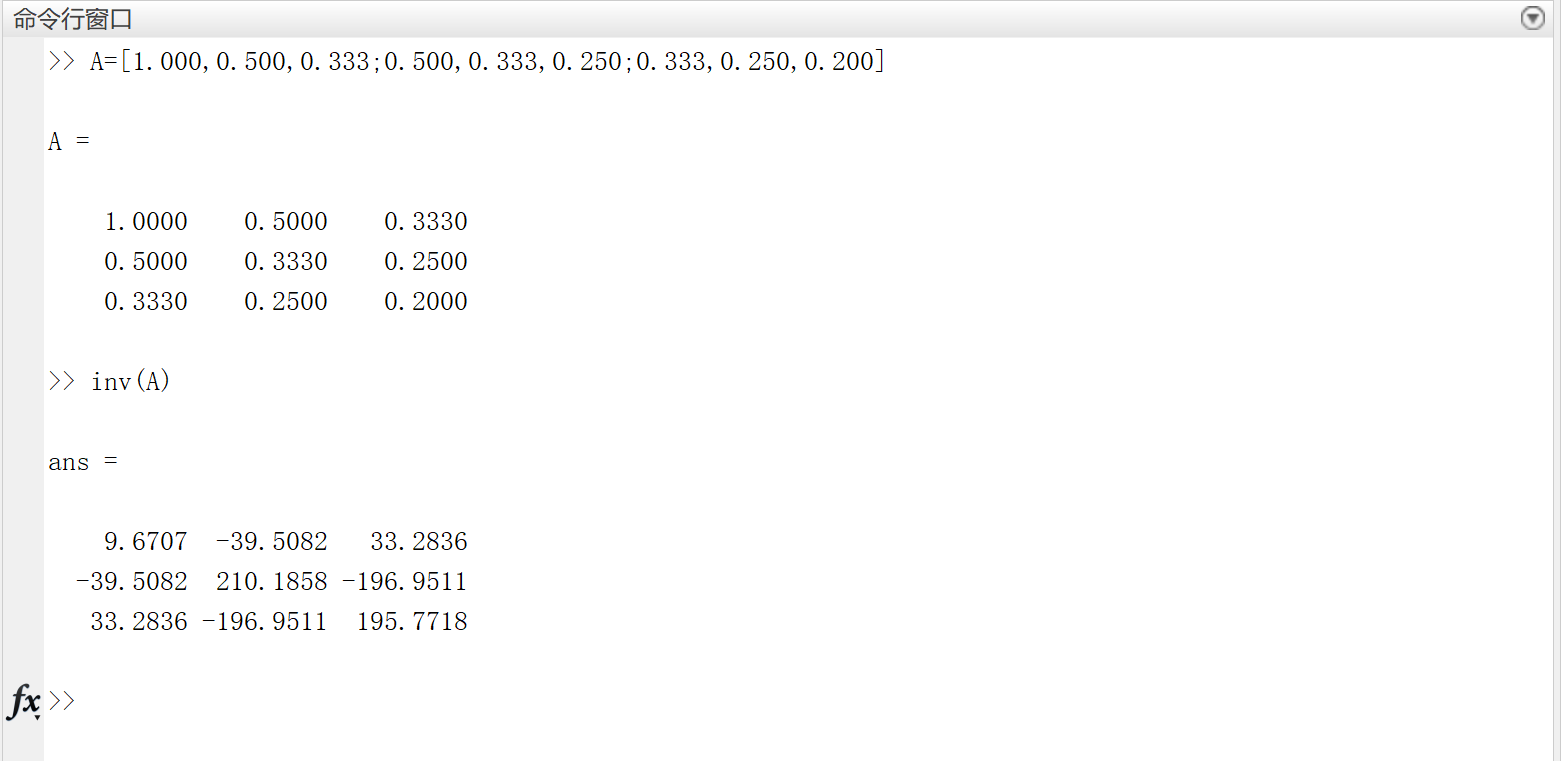
\includegraphics[width=1.3\textwidth]{1.png}
  \caption{ }
  \label{fig:1.5.11}
\end{figure}
\end{solution}
\begin{question}
  比较在直接消去和列选主元消去之下,矩阵
$$
A=
\begin{pmatrix}
  0.001&0\\
1&1000
\end{pmatrix}
$$
的主元(这是一个在进行消去之前就需加大主元的例子).
\end{question}
\begin{solution}
如果采用列选主元消去法,则过程为
$$
\begin{pmatrix}
  1&0\\
-0.001&1
\end{pmatrix}
\begin{pmatrix}
  0&1\\
1&0
\end{pmatrix}
\begin{pmatrix}
  0.001&0\\
1&1000
\end{pmatrix}=
\begin{pmatrix}
  1&1000\\
0&-1
\end{pmatrix}.
$$
如果采用直接消元法,则过程为
$$
\begin{pmatrix}
  1&0\\
-1000&1
\end{pmatrix}
\begin{pmatrix}
  0.001&0\\
1&1000
\end{pmatrix}=
\begin{pmatrix}
  0.001&0\\
0&1000
\end{pmatrix}.
$$
\end{solution}
\begin{question}
  试解释为什么在列选主元之下,$L$中的$l_{i,j}$都满足$|l_{i,j}|\leq
  1$.试证明:如果$A$的元素满足$|a_{ij}|\leq 1$,那么第一步消去(变第一列
  主元下面的元素为零)之后,所有元素都以$2$为界;第$k$步消去后,所有元
  素都以$2^k$为界.请构造一个$3\times 3$的$A$,使得$|a_{ij}|\leq
  1$,$|l_{ij}|\leq 1$,最后一个主元为$4$.
\end{question}
\begin{solution}
 理由显然,略叙.我只构造出满足题意的矩阵.
\begin{align*}
A=\begin{pmatrix}
1  & 1&-1 \\
-1&0&-1      \\
-1&1&1
\end{pmatrix}\Rightarrow
      \begin{pmatrix}
        1&1&-1\\
0&1&-2 \\
0&2&0
      \end{pmatrix}\Rightarrow
      \begin{pmatrix}
        1&1&-1\\
0&1&-2\\
0&0&4
      \end{pmatrix}
\end{align*}
\end{solution}
\section{带状矩阵,对称矩阵及其应用}
\begin{question}
  将我们刚举过的这个例子中的$a_{11}=2$改为$a_{11}=1$,求新三对角矩阵的分
  解式LDU.
\end{question}
\begin{solution}
  即求矩阵
$$
\begin{pmatrix}
  1&-1&0&0&0\\
  -1&2&-1&0&0\\
  0&-1&2&-1&0\\
  0&0&-1&2&-1\\
  0&0&0&-1&2
\end{pmatrix}
$$
的LDU分解.
\begin{align*}
  &
    \begin{pmatrix}
      1&0&0&0&0\\
      0&1&0&0&0\\
      0&0&1&0&0\\
      0&0&0&1&0\\
      0&0&0&1&1
    \end{pmatrix}
               \begin{pmatrix}
                 1&0&0&0&0\\
                 0&1&0&0&0\\
                 0&0&1&0&0\\
                 0&0&1&1&0\\
                 0&0&0&0&1
               \end{pmatrix}\\&
                                \begin{pmatrix}
                                  1&0&0&0&0\\
                                  0&1&0&0&0\\
                                  0&1&1&0&0\\
                                  0&0&0&1&0\\
                                  0&0&0&0&1
                                \end{pmatrix}
                                           \begin{pmatrix}
                                             1&0&0&0&0\\
                                             1&1&0&0&0\\
                                             0&0&1&0&0\\
                                             0&0&0&1&0\\
                                             0&0&0&0&1
                                           \end{pmatrix}
                                                      \begin{pmatrix}
                                                        1&-1&0&0&0\\
                                                        -1&2&-1&0&0\\
                                                        0&-1&2&-1&0\\
                                                        0&0&-1&2&-1\\
                                                        0&0&0&-1&2
                                                      \end{pmatrix}\\&=
                                                                       \begin{pmatrix}
                                                                         1&-1&0&0&0\\
                                                                         0&1&-1&0&0\\
                                                                         0&0&1&-1&0\\
                                                                         0&0&0&1&-1\\
                                                                         0&0&0&0&1
                                                                       \end{pmatrix}
\end{align*}
确定了U之后,L便不必求.直接得到矩阵的LDU分解为
$$
\begin{pmatrix}
  1&0&0&0&0\\
  -1&1&0&0&0\\
  0&-1&1&0&0\\
  0&0&-1&1&0\\
  0&0&0&-1&1
\end{pmatrix}
\begin{pmatrix}
  1&0&0&0&0\\
  0&1&0&0&0\\
  0&0&1&0&0\\
  0&0&0&1&0\\
  0&0&0&0&1
\end{pmatrix}
\begin{pmatrix}
  1&-1&0&0&0\\
  0&1&-1&0&0\\
  0&0&1&-1&0\\
  0&0&0&1&-1\\
  0&0&0&0&1
\end{pmatrix}.
$$
\end{solution}
\begin{question}
  试消去对称矩阵
$$
A=
\begin{pmatrix}
  a&b&c\\
  b&d&e\\
  c&e&g
\end{pmatrix}
$$
中主元$a$正下方的各元素.验证经这一步消去之后,得到的矩阵$B$的右
下$2\times 2$矩阵依旧是对称的.由此认识每一步消去都不改变对称性.
\end{question}
\begin{solution}
  首先,规定记号.对于任意一个矩阵$A$来说,将矩阵$A$的第$i$行加上第$j$行
  的$l_{ij}$倍,是一种初等行变换,变换矩阵记为$E_{ij}$,矩阵$A$经过这样的
  变换得到的矩阵记为$E_{ij}A$.将矩阵$A$的第$i$列加上第$j$列的$l_{ij}$倍,
  是一种初等列变换,矩阵$A$经过这样的初等列变换的作用,得到
  的矩阵不必用新的符号来表示,而易得为$(E_{ij}A^{T})^T=AE_{ij}^T$.\\

  下面我们来证明,如果$A$是一个对称矩阵,则将矩阵$A$的第$i$行加上
  第$j$行的$q$倍,再将得到的矩阵的第$i$列加上第$j$列的$q$倍,最终得到的
  矩阵依然是一个对称矩阵,这是因为最终得到的矩阵
  为$(E_{ij}A)E_{ij}^T=E_{ij}AE_{ij}^{T}$,而将该矩阵进行转置后,得到
$$
(E_{ij}AE_{ij}^{T})^T=E_{ij}A^TE_{ij}^{T}=E_{ij}AE_{ij}^T.
$$
即,最终得到的矩阵经过转置后是其本身,因此最终得到的矩阵是对称矩阵.\\

下面利用这个结论来做题目.先将矩阵的第$2$行加上第$1$行的倍
数,{\color{red}使得矩阵$A$的第二行首项为$0$}.再将矩阵的第$2$列加上
第$1$列的倍数,使得矩阵的第$2$列首项为$0$.由上面的结论,这样做得到的矩
阵是对称矩阵.然后再继续操作,将矩阵的第$3$行加上矩阵的第$1$行的倍
数,{\color{red}使得第三行首项为$0$},再将第三列加上第$1$列的倍数,使得
矩阵的第三列首项为$0$.最终得到的矩阵依然是对称矩阵.而且最终得到的对称矩
阵的右下$2\times
2$矩阵和矩阵$B$的右下$2\times 2$矩阵必定是同一个矩阵(想一想为什么?注意
红色的字),因此矩阵$B$的右下$2\times 2$矩阵是对称矩阵.
\end{solution}
\begin{question}
  求逼近
$$
- \frac{d^2u}{dx^2}=f(x),\frac{du}{dx}(0)=\frac{du}{dx}(1)=0
$$
的$5\times 5$矩阵$A$,边界条件换为$u_0=u_1,u_6=u_{5}$.证明所得矩阵作用
于常数向量$(1,1,1,1,1)$,结果为零.$A$是奇异矩阵.类似地,再证明如果
$u(x)$是连续问题的解,那么$u(x)+1$也是.题给的边界条件去不掉$C+Dx$的不
确定性,因而解不唯一.
\end{question}
\begin{solution}
 将该连续问题离散化.即,
\begin{align*}
-u_{0}+2u_1-u_2&=h^2f(x_1)\\
-u_1+2u_2-u_3&=h^2f(x_2)\\
-u_2+2u_3-u_4&=h^2f(x_3)\\
-u_3+2u_4-u_5&=h^2f(x_4)\\
-u_4+2u_5-u_6&=h^2f(x_5)\\
\end{align*}
由于$u_0=u_1,u_5=u_6$,因此上面的方程组可以化为
\begin{align*}
  u_1-u_2&=h^2f(x_1)\\
-u_1+2u_2-u_3&=h^2f(x_2)\\
-u_2+2u_3-u_4&=h^2f(x_3)\\
-u_3+2u_4-u_5&=h^2f(x_4)\\
-u_4+u_5&=h^2f(x_5)\\
\end{align*}
写成矩阵形式,即
$$
\begin{pmatrix}
1&-1&0&0&0\\
-1&2&-1&0&0\\
0&-1&2&-1&0\\
0&0&-1&2&-1\\
0&0&0&-1&1
\end{pmatrix}
\begin{pmatrix}
u_1\\
u_2\\
u_3\\
u_4\\
u_5\\
\end{pmatrix}=h^{2}
\begin{pmatrix}
f(x_1)\\
f(x_2)\\
f(x_3)\\
f(x_4)\\
f(x_5)\\
\end{pmatrix}
$$
其余略.
\end{solution}
\begin{question}
  $h=\frac{1}{4}$,$f(x)=4\pi^2\sin 2\pi x$时差分方程(29)为
$$
\begin{pmatrix}
  2&-1&0\\
 -1&2&-1\\
0&-1&2
\end{pmatrix}
\begin{pmatrix}
  u_1\\
u_2\\
u_3
\end{pmatrix}=\frac{\pi^2}{4}
\begin{pmatrix}
  1\\
0\\
-1
\end{pmatrix}.
$$
解出$u_i$,并将求得的解与真解$u=\sin 2\pi x$在
$x=\frac{1}{4}$,$x=\frac{1}{2}$,$x=\frac{3}{4}$处的值相比较,算出误差.
\end{question}
\begin{solution}
将系数矩阵进行LU分解可得
$$
\begin{pmatrix}
  2&-1&0\\
-1&2&-1\\
0&-1&2
\end{pmatrix}=
\begin{pmatrix}
  1&0&0\\
-\frac{1}{2}&1&0\\
0&0&1
\end{pmatrix}
\begin{pmatrix}
  1&0&0\\
0&1&0\\
0&\frac{-2}{3}&1
\end{pmatrix}
\begin{pmatrix}
  2&-1&0\\
0&\frac{3}{2}&-1\\
0&0&\frac{4}{3}
\end{pmatrix}=
\begin{pmatrix}
  1&0&0\\
\frac{-1}{2}&1&0\\
0&\frac{-2}{3}&1
\end{pmatrix}
\begin{pmatrix}
  2&-1&0\\
0&\frac{3}{2}&-1\\
0&0&\frac{4}{3}
\end{pmatrix}.
$$
所以差分方程的解
$$
\begin{pmatrix}
  u_1\\
u_2\\
u_3
\end{pmatrix}=
\begin{pmatrix}
  \frac{1}{3}\\
\frac{-1}{3}\\
-1
\end{pmatrix}.
$$而真解为$(1,0,-1)^{T}$.误差计算就算了,好像离得挺远.
\end{solution}
\section{复习题}
\begin{question}
  试对矩阵
$$
A=
\begin{pmatrix}
  1&0\\
  1&1
\end{pmatrix},B=
\begin{pmatrix}
  1&1\\
  0&1
\end{pmatrix}
$$
计算$A+B$和$AB$.
\end{question}
\begin{solution}
$$
A+B=
\begin{pmatrix}
  2&1\\
  1&2
\end{pmatrix}.
$$
$$
AB=
\begin{pmatrix}
  1&1\\
  1&2
\end{pmatrix}
$$
\end{solution}
\begin{question}
  对上题矩阵计算$A^{-1},B^{-1}$和$(AB)^{-1}$.
\end{question}
\begin{solution}
  $A^{-1}=
  \begin{pmatrix}
    1&0\\
    -1&1
  \end{pmatrix},B^{-1}=
  \begin{pmatrix}
    1&-1\\
    0&1
  \end{pmatrix}.  $
$$
(AB)^{-1}=B^{-1}A^{-1}=
\begin{pmatrix}
  2&-1\\
  -1&1
\end{pmatrix}.
$$
\end{solution}
\begin{question}
  用正向消去和反向代入解
  \begin{align*}
    2u-3v~~~~~~&=8\\
    4u-5v+w&=15\\
    2u~~~~~~+4w&=1
  \end{align*}
\end{question}
\begin{solution}
  先将系数矩阵
$$
A=
\begin{pmatrix}
  2&-3&0\\
  4&-5&1\\
  2&0&4
\end{pmatrix}
$$
化为上三角矩阵.
$$
\begin{pmatrix}
  1&0&0\\
  0&1&0\\
  0&-3&1
\end{pmatrix}
\begin{pmatrix}
  1&0&0\\
  0&1&0\\
  -1&0&1
\end{pmatrix}
\begin{pmatrix}
  1&0&0\\
  -2&1&0\\
  0&0&1
\end{pmatrix}
\begin{pmatrix}
  2&-3&0\\
  4&-5&1\\
  2&0&4
\end{pmatrix}=
\begin{pmatrix}
  2&-3&0\\
  0&1&1\\
  0&0&1
\end{pmatrix}.
$$
所以
$$
A=LU=
\begin{pmatrix}
  1&0&0\\
  2&1&0\\
  0&0&1
\end{pmatrix}
\begin{pmatrix}
  1&0&0\\
  0&1&0\\
  1&0&1
\end{pmatrix}
\begin{pmatrix}
  1&0&0\\
  0&1&0\\
  0&3&1
\end{pmatrix}
\begin{pmatrix}
  2&-3&0\\
  0&1&1\\
  0&0&1
\end{pmatrix}=
\begin{pmatrix}
  1&0&0\\
  2&1&0\\
  1&3&1
\end{pmatrix}
\begin{pmatrix}
  2&-3&0\\
  0&1&1\\
  0&0&1
\end{pmatrix}.
$$
正向消去的过程即为$L^{-1}(8,15,1)^T$,即为
$$
\begin{pmatrix}
  1&0&0\\
  0&1&0\\
  0&-3&1
\end{pmatrix}
\begin{pmatrix}
  1&0&0\\
  0&1&0\\
  -1&0&1
\end{pmatrix}
\begin{pmatrix}
  1&0&0\\
  -2&1&0\\
  0&0&1
\end{pmatrix}
\begin{pmatrix}
  8\\
  15\\
  1
\end{pmatrix}=
\begin{pmatrix}
  8\\
  -1\\
  -4
\end{pmatrix}.
$$
反向代入的过程即为解
$$
\begin{pmatrix}
  2&-3&0\\
  0&1&1\\
  0&0&1
\end{pmatrix}
\begin{pmatrix}
  u\\
  v\\
  w
\end{pmatrix}=
\begin{pmatrix}
  8\\
  -1\\
  -4
\end{pmatrix}
$$
的过程,解得
$$
\begin{pmatrix}
  u\\
  v\\
  w
\end{pmatrix}=
\begin{pmatrix}
  \frac{17}{2}\\
  3\\
  -4
\end{pmatrix}.
$$
\end{solution}
\begin{question}
  将上题的系数矩阵分解为$A=LU$.
\end{question}
\begin{solution}
  在上题的解答中已经完成.
\end{solution}
\begin{question}
  一个三个方程的方程组已给,试写出矩阵$E$,它能起到从第三个方程减去第二
  个方程的作用.
\end{question}
\begin{solution}
 $$ 
 E=
 \begin{pmatrix}
   1&0&0\\
   0&1&0\\
   0&-1&1
 \end{pmatrix}.
 $$
\end{solution}
\begin{question}
  试写出$3\times 3$矩阵$P$,它能起到交换一、三两个方程的作用.
\end{question}
\begin{solution}
  $$ 
  P=
  \begin{pmatrix}
    0&0&1\\
    0&1&0\\
    1&0&0\\
  \end{pmatrix}.
 $$
\end{solution}
\begin{question}
  什么样的$3\times 3$矩阵能起到乘第二个方程以$-1$,保持另外两个方程不变
  的作用.
\end{question}
\begin{solution}
 $$ 
 \begin{pmatrix}
   1&0&0\\
   0&-1&0\\
   0&0&1
 \end{pmatrix}
 $$
\end{solution}
\begin{question}
  试用消去法判断下面的方程组是否有解
  \begin{align*}
    u+v+w&=0\\
    u+2v+3w&=0\\
    3u+5v+7w&=1
  \end{align*}
\end{question}
\begin{solution}
  尝试将系数矩阵$A=
  \begin{pmatrix}
    1&1&1\\
    1&2&3\\
    3&5&7
  \end{pmatrix}
  $进行分解.可得
$$
A=
\begin{pmatrix}
  1&0&0\\
  1&1&0\\
  0&0&1
\end{pmatrix}
\begin{pmatrix}
  1&0&0\\
  0&1&0\\
  3&0&1
\end{pmatrix}
\begin{pmatrix}
  1&0&0\\
  0&1&0\\
  0&2&1
\end{pmatrix}
\begin{pmatrix}
  1&1&1\\
  0&1&2\\
  0&0&0
\end{pmatrix}=
\begin{pmatrix}
  1&0&0\\
  1&1&0\\
  3&2&1
\end{pmatrix}
\begin{pmatrix}
  1&1&1\\
  0&1&2\\
  0&0&0
\end{pmatrix}=LU.
$$
正向消去可得
$$
L^{-1}(0,0,1)^{T}=(0,0,1)^T.
$$
所以可得$0u+0v+0w=1$,无解!
\end{solution}
\begin{question}
  试用消去法和行交换解
  \begin{align*}
    u+v-w&=2\\
    3u+3v+w&=2\\
    u~~~~~~+w&=0.
  \end{align*}
\end{question}
\begin{solution}
  将系数矩阵
$$
A=
\begin{pmatrix}
  1&1&-1\\
  3&3&1\\
  1&0&1
\end{pmatrix}
$$
进行分解.可得
$$
\begin{pmatrix}
  1&0&0\\
  0&0&1\\
  0&1&0
\end{pmatrix}
\begin{pmatrix}
  1&0&0\\
  0&1&0\\
  -1&0&1
\end{pmatrix}
\begin{pmatrix}
  1&0&0\\
  -3&1&0\\
  0&0&1
\end{pmatrix}
\begin{pmatrix}
  1&1&-1\\
  3&3&1\\
  1&0&1
\end{pmatrix}=
\begin{pmatrix}
  1&1&-1\\
  0&-1&2\\
  0&0&4
\end{pmatrix}.
$$
当然,可以将行交换的矩阵最先作用于矩阵$A$.
$$
PA=
\begin{pmatrix}
  1&0&0\\
  0&0&1\\
  0&1&0
\end{pmatrix}
\begin{pmatrix}
  1&1&-1\\
  3&3&1\\
  1&0&1
\end{pmatrix}=
\begin{pmatrix}
  1&1&-1\\
  1&0&1\\
  3&3&1
\end{pmatrix}.
$$
将矩阵PA化为上三角矩阵,即
$$
E_{3,1}E_{2,1}PA=U,\mbox{即}L^{-1}PA=U,
$$
即
$$
\begin{pmatrix}
  1&0&0\\
  0&1&0\\
  -3&0&1
\end{pmatrix}
\begin{pmatrix}
  1&0&0\\
  -1&1&0\\
  0&0&1
\end{pmatrix}
\begin{pmatrix}
  1&1&-1\\
  1&0&1\\
  3&3&1
\end{pmatrix}=
\begin{pmatrix}
  1&1&-1\\
  0&-1&2\\
  0&0&4
\end{pmatrix}.
$$
所以$A=P^{-1}LU=PLU$.进行正向消去和反向代入解得$(u,v,w)=(1,0,-1)$.
\end{solution}
\begin{question}
  试分解
$$
A=
\begin{pmatrix}
  1&4&0\\
  0&1&0\\
  0&3&1
\end{pmatrix}
$$
为LU.
\end{question}
\begin{solution}
 $$ 
 \begin{pmatrix}
   1&0&0\\
   0&1&0\\
   0&-3&1
 \end{pmatrix}
 \begin{pmatrix}
   1&4&0\\
   0&1&0\\
   0&3&1
 \end{pmatrix}=
 \begin{pmatrix}
   1&4&0\\
   0&1&0\\
   0&0&1
 \end{pmatrix}.
 $$
 所以
$$
A=
\begin{pmatrix}
  1&0&0\\
  0&1&0\\
  0&3&1
\end{pmatrix}
\begin{pmatrix}
  1&4&0\\
  0&1&0\\
  0&0&1
\end{pmatrix}.
$$
\end{solution}
\begin{question}
  求
$$
\begin{pmatrix}
  2&3\\
  3&4
\end{pmatrix}
$$
的逆矩阵.
\end{question}
\begin{solution}
$$
  \begin{pmatrix}
    2&3&1&0\\
    3&4&0&1
  \end{pmatrix}\to
  \begin{pmatrix}
    2&3&1&0\\
    0&-\frac{1}{2}&-\frac{3}{2}&1
  \end{pmatrix}\to
  \begin{pmatrix}
    2&0&-8&6\\
    0&\frac{-1}{2}&\frac{-3}{2}&1
  \end{pmatrix}\to
  \begin{pmatrix}
    1&0&-4&3\\
    0&1&3&-2
  \end{pmatrix}.
$$
所以题中矩阵的逆矩阵为$
\begin{pmatrix}
  -4&3\\
  3&-2
\end{pmatrix}.  $
\end{solution}
\begin{question}
  一个$3\times 3$矩阵,它的任何一行都不是另外一行的倍数.问该矩阵是否一
  定有逆矩阵?请举例.
\end{question}
\begin{solution}
  不一定.比如$
  \begin{pmatrix}
    1&4&7\\
    2&5&8\\
    3&6&9
  \end{pmatrix}.  $该矩阵的第三列是第一列加上第二列得到的,该矩阵不可
  逆.这是因为,这样的矩阵在进行初等行变换后,“第三列是第一列加上第二列
  得到的”这个性质始终保持不变,假如可逆,在进行一系列初等行变换后可以
  变成单位矩阵,但是单位矩阵不满足这个性质.矛盾.所以该矩阵不可逆.
\end{solution}
\begin{question}
  用Gauss-Jordan法求
$$
A=
\begin{pmatrix}
  1&1&0\\
  0&1&1\\
  0&0&1
\end{pmatrix}
$$
的逆矩阵.
\end{question}
\begin{solution}
  \begin{align*}
    \begin{pmatrix}
      1&1&0&1&0&0\\
      0&1&1&0&1&0\\
      0&0&1&0&0&1
    \end{pmatrix}\to
                 \begin{pmatrix}
                   1&1&0&1&0&0\\
                   0&1&0&0&1&-1\\
                   0&0&1&0&0&1
                 \end{pmatrix}\to
                              \begin{pmatrix}
                                1&0&0&1&-1&1\\
                                0&1&0&0&1&-1\\
                                0&0&1&0&0&1
                              \end{pmatrix}
  \end{align*}
所以$A$的逆矩阵为$
\begin{pmatrix}
  1&-1&1\\
0&1&-1\\
0&0&1
\end{pmatrix}.
$
\end{solution}
\begin{question}
试解释为什么三角阵的逆矩阵也是三角阵.
\end{question}
\begin{solution}
 用Gauss-Jordan法易得下三角矩阵的逆矩阵是下三角矩阵,上三角矩阵的逆矩
 阵是上三角矩阵.
\end{solution}
\begin{question}
  设$E$是一个$2\times 2$矩阵,它起到加第一个方程到第二个方程上去的作用.问
  $E^{50}$起到什么作用?试写出$E,E^{50}$和$50E$.
\end{question}
\begin{solution}
  $E^{50}$的作用是加第一个方程的50倍到第二个方程上去.
$$
E=
\begin{pmatrix}
  1&0\\
1&1
\end{pmatrix},E^{50}=
\begin{pmatrix}
  1&0\\
50&1
\end{pmatrix},50E=
\begin{pmatrix}
  50&0\\
50&50
\end{pmatrix}.
$$
\end{solution}
\begin{question}
  试写出一个有无穷多解的$2\times 2$方程组.
\end{question}
\begin{solution}
$$
\begin{cases}
  x+y=1\\
2x+2y=2
\end{cases}.
$$
\end{solution}
\end{document}
